\documentclass[aspectratio=169,t]{beamer}
\usepackage[utf8]{inputenc}
\usepackage[T1]{fontenc}


\title{Einführung in die Gesundheits\-informatik}
\date{WS 2019/2020}
\author[PWD]{Dr.-Ing. Piotr Wojciech Dabrowski}

\usepackage{HTWBeamerTemplate/beamerthemeHTW}
\addbibresource{Bilder/imagesources.bib}
\begin{document}

\stepcounter{slidesection}
\setbeamertemplate{background}[bgfirst]
\setbeamertemplate{footline}[first]
\subtitle{\theslidesection: Allgemeines}
\titlegraphic{Bilder/logo.png}
\begin{frame}[noframenumbering]
\titlepage
\begin{textblock}{10}(4.75,15)
\cite{EinfuehrungLogo}
\end{textblock}
\end{frame}
\setbeamertemplate{footline}[presentationbody] 
\setbeamertemplate{background}[bgbody]

\begin{frame}{Vorstellung}
    \note<4->{
        Erstes Mal Vorlesung, Background nicht in mobilen Applikationen\\Bitte um Geduld, Hinweise\\
        Whiteboard:
        \begin{itemize}
            \item Wer nicht aufgerufen werden will, nach der VL bei mir melden (stelle keine Fragen) oder X oben links bei Antwort
            \item Strichliste: Nur für mich für Gleichmäßigkeit, nicht zensurrelevant
            \item Spontanes, prägnantes, kohärentes Sprechen wichtig! Beispiel: Empfehlung an Politikerin
        \end{itemize}
    }
 \begin{itemize}
     \item<2-> Kurz zu mir
     \only<2-5>{
      \begin{itemize}
        \item<2-5> Kontakt: Piotr.Dabrowski@htw-berlin.de - gerne nutzen!
        \item<2-5> Github: https://github.com/dabrowskiw/
        \item<3-5> Geboren 1981 in Warschau
        \item<3-5> Studium der Biotechnologie \& Informatik an der TU Berlin
        \item<3-5> Promotion über Auswertung von Hochdurchsatzdaten für Virus-Diagnostik
        \item<3-5> Aufbau der bioinformatischen Analytik für das NGS-Labor des RKI
        \item<3-5> Aufbau der Bioinformatics Core Facility am RKI
        \note<3>{Entsprechend andere Schwerpunkte der VL, als bisher\\Gesundheitsinformatik ist nicht gleich Bioinformatik!}
        \item<4-5> Seit WS 2019/2020 an der HTW
        \note<4>{Erste Vorlesungen an der HTW:
            \begin{itemize}
                \item Lerne erst Modalitäten kennen
                \item Kenne die Vorkenntnisse/präferierte Art der Studierenden nicht
                \item Primäres Ziel: Verständnis aufbauen, "durch den Stoff kommen" zweitrangig
                \item Also bitte (rechtzeitig) melden, wenn Interesse an Vertiefung besteht
                \item Gemeinsame Reise - bitte immer melden, wenn was ist!
                \item Gerne auch außerhalb der Sprechzeiten, wenn die Tür offen ist einfach reinkommen.
            \end{itemize}
        }
        \item<5> Hang zum Experimentieren in der Vorlesung - Feedback erwünscht!
        \note<5>{
        \begin{itemize}
            \item Gruppenarbeiten
            \item Mini-Whiteboards
            \item Angebot: Treppenlauf
            \item Bitte melden, wenn es zu viel wird!
        \end{itemize}}
      \end{itemize}
     }
     \item<6-> Der Todesstern \& (ausgewählte) andere Hilfsmittel
     \item<10-> Sie \& Ihre Vorstellungen von der Gesundheitsinformatik
     \note<10>{
     Ziele:
     \begin{itemize}
         \item Kennenlernen der Vorkenntnisse und Wünsche
         \item Eventuell Anpassung der Schwerpunkte später im Semester
         \item Eigene Auseinandersetzung hilft beim Erinnern
         \item Aber erst mal Allgemeines fertig, dann dieser Teil der Vorstellung!
     \end{itemize}
     }
 \end{itemize}
 \only<6-9>{
  \begin{textblock}{15}(2,7)
   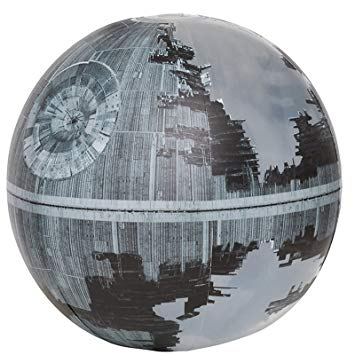
\includegraphics[width=3cm]{Bilder/Todesstern.jpg}
  \end{textblock}
 }
 \only<7-9>{
  \begin{textblock}{15}(5.5,8.25)
   
\includegraphics[width=3cm]{Bilder/Tischnamensschild.png}
  \end{textblock}
 }
 \only<8-9>{
  \begin{textblock}{15}(9,7.5)
   
\includegraphics[angle=77,origin=c,height=2cm]{Bilder/Tischnamensschild.png}
  \end{textblock}
 }
 \only<9>{
  \begin{textblock}{15}(11.5,8)
   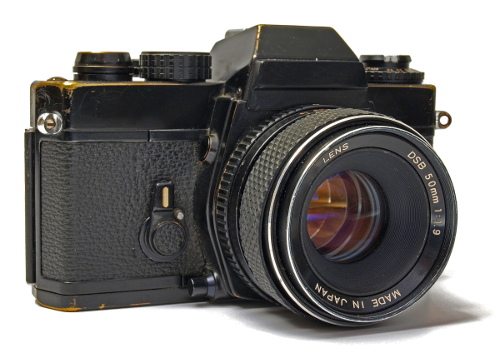
\includegraphics[width=3cm]{Bilder/DSLR.png}
  \end{textblock}
 }
\end{frame}

\begin{frame}{Inhalt der Vorlesung}
 Was macht Informatik im Gesundheitswesen? \uncover<2->{Am Beispiel eines Patienten mit Tuberkulose oder Krebs.}
\note<2>{
 \begin{itemize}
     \item Differentialdiagnostik z.T. interessant, werden wir gleich sehen.
     \item Generell drei Aspekte:
     \begin{itemize}
         \item Gesundheitswesen/Diagnostik/Einsatz im Krankenhaus
         \item Biologische Grundlagen
         \item Programmierung
     \end{itemize}
 \end{itemize}
}
 \begin{itemize}
     \item<3-> Gesundheitssystem allgemein
     \only<3>{\begin{itemize}
        \item Wo kommt das Geld für die Behandlung her?
        \item Wer regelt was wann wie gemacht wird?
        \item Welche Daten werden wo gespeichert? 
     \end{itemize}}
     \item<4-> Molekulare Diagnostik
     \only<4>{\begin{itemize}
        \item Erregernachweise (ELISA, PCR)
        \item Grundlagen der Arbeit mit Bilddaten
     \end{itemize}}     
     \item<5-> Bildgebende Verfahren
     \only<5>{\begin{itemize}
        \item Blick in das Gewebe: Ultraschall, Röntgen, \\CT, MRT, OCT
        \item Ein wenig Mathematik (Fourier-Transformation)
        \item Fortgeschrittenere Bilddatenverarbeitung
     \end{itemize}}     
     \item<6-> DNA-basierte Hochdurchsatz-Diagnostik
     \only<6>{\begin{itemize}
        \item Microarrays, Next Generation Sequencing
        \item Einige Methoden des maschinellen Lernens
        \item Krebsdiagnostik
     \end{itemize}}     
     \item<7-> Proteomik
     \only<7>{\begin{itemize}
        \item Tandem-MS
        \item Wie sicher ist man sich, es falsch \\gemacht zu haben?
        \item Verbesserte Krebsdiagnostik
     \end{itemize}}     
 \end{itemize}
 \only<3>{
  \begin{textblock}{10}(7.5,4.5)
   \begin{figure}[h!]
     \label{figure:VDEK}
     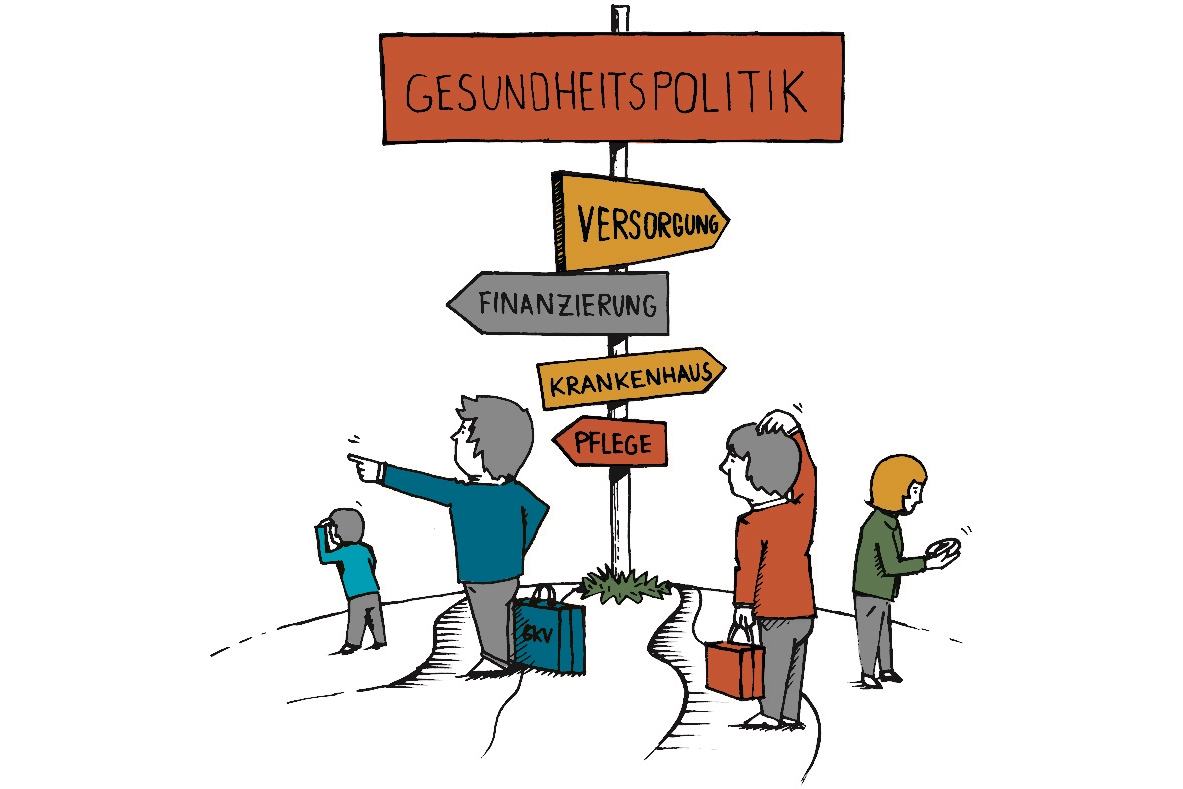
\includegraphics[width=7.5cm]{Bilder/Gesundheitspolitik.png}
     \caption{Cartoon von VDEK \cite{VDEK}}
   \end{figure}
  \end{textblock}
 }
 \addtocounter{figure}{1}
 \only<4>{
  \begin{textblock}{10}(7,4.5)
   \begin{figure}[h!]
     \label{figure:ELISA}
     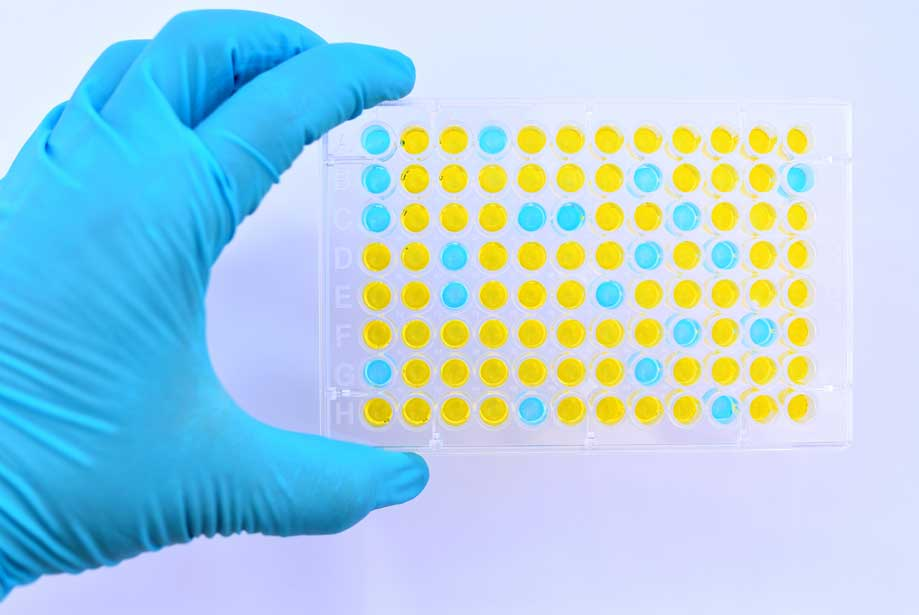
\includegraphics[width=7.5cm]{Bilder/ELISA.jpg}
     \caption{ELISA-Platte \cite{ELISA}}
   \end{figure}
  \end{textblock}
 }
 \addtocounter{figure}{1}
 \only<5>{
  \begin{textblock}{10}(7.5,4.5)
   \begin{figure}[h!]
     \label{figure:CT}
     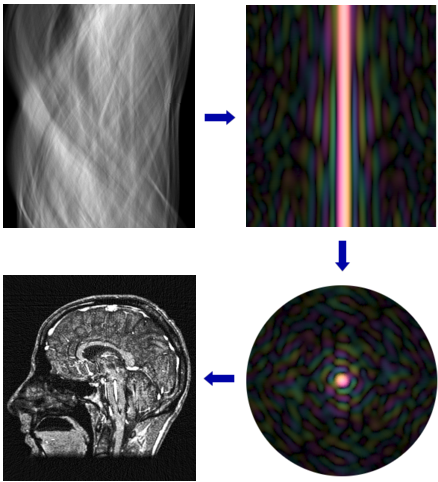
\includegraphics[width=4.5cm]{Bilder/CT.png}
     \caption{Radon-Transformation \cite{Radon}}
   \end{figure}
  \end{textblock}
 }
 \addtocounter{figure}{1}
 \only<6>{
  \begin{textblock}{10}(7.5,4.5)
   \begin{figure}[h!]
     \label{figure:NGS}
     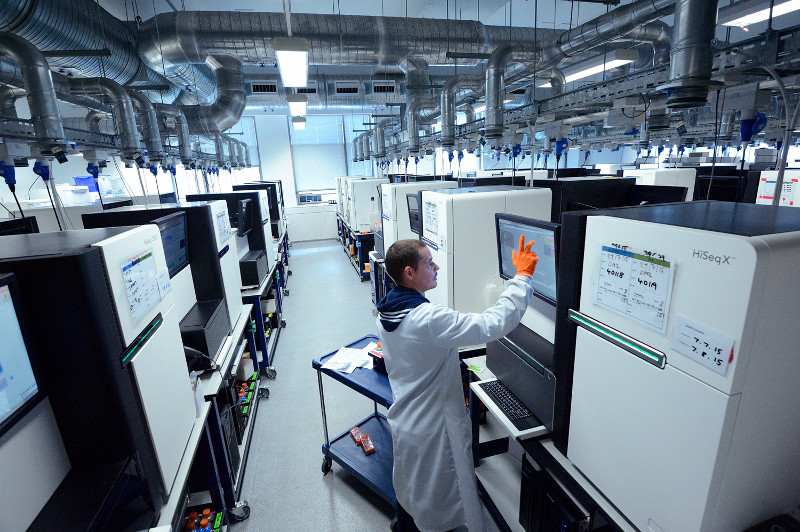
\includegraphics[width=6.5cm]{Bilder/NGS.jpg}
     \caption{NGS-Labor am Sanger Institute \cite{NGS}}
   \end{figure}
  \end{textblock}
 }
 \addtocounter{figure}{1}
 \only<7>{
  \begin{textblock}{10}(7,4.5)
   \begin{figure}[h!]
     \label{figure:HPLCMS}
     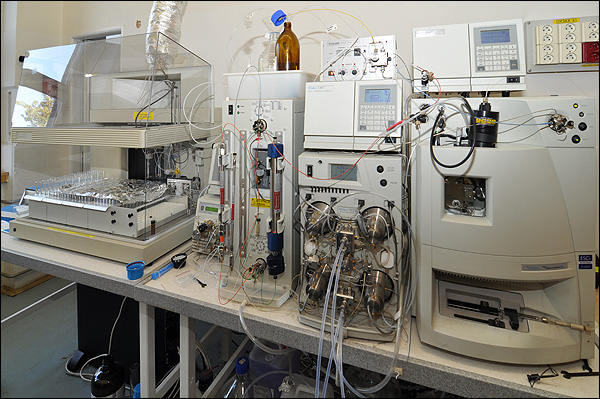
\includegraphics[width=6.5cm]{Bilder/LCMS.jpg}
     \caption{Ein (älteres) Massenspektrometer \cite{LCMS}}
   \end{figure}
  \end{textblock}
 }
\end{frame}

\begin{frame}{Inhalt der Übung}
 \begin{itemize}
     \item Firmenbesuche
     \only<2>{
      \begin{itemize}
        \item VmScope GmbH
	\item Berlin Heart GmbH (KW45)
        \item RKI (NGS-Lab, Proteomik \& Bioinformatik)
	\item Weitere?
      \end{itemize}
     }
     \note<2>{
       Zur Steigerung der Aufmerksamkeit: Kurztestate nach Besuch der Firmen, 2-3 Fragen zur Firma auf max. 1/2 A4-Seite zu beantworten.
     }
     \item Softwareentwicklung basierend auf Vorlesungs-Inhalten
     \item Kurzvorstellungen der Übungsergebnisse
 \end{itemize}
\end{frame}

%\begin{frame}{Gesamtfahrplan (vorläufig)}
%  \note{Vorläufig, je nach:
%   \begin{itemize}
%       \item Allgemeinem Vorankommen (gründlich verstehen wichtiger als kompletten Stoff durchprügeln)
%       \item Terminverschiebungen bei Firmen
%   \end{itemize}
%  }
%  \begin{columns}
%   \begin{column}{0.5\textwidth}
%  \begin{itemize}
%    \item KW41: Gesundheitssystem
%    \item KW42: Molekulare Diagnostik % und Grundlagen Python
%    \item KW43: Ü: Datenauswertung in Python
%    \item KW44: Ü: Datenauswertung in Python
%    \item KW45: Besuch: Berlin Heart
%    \item KW46: Bildgebende Verfahren
%    \item KW47: Besuch: VmScope
%    \item KW48: Ü: Bilddatenauswertung
%  \end{itemize}
%   \end{column}
%   \begin{column}{0.5\textwidth}
%  \begin{itemize}
%    \item KW50: Besuch: MicroDiscovery
%    \item KW51: Ü: Microarray-Auswertung
%    \item KW02: NGS
%    \item KW03: Besuch: RKI
%    \item KW04: Ü: NGS-Auswertung
%    \item KW05: Ergebnisvorstellung
%%    \item KW50: 
%%    \item KW50: 
%%    \item KW44: Python-Grundlagen, Auswertung von Daten aus molekularer Diagnostik
%%    \item KW46: Fortgeschrittenere Bilddaten-Auswertung
%%    \item KW48: Besuch der MicroDiscovery GmbH (Auftragsdatenauswertung, Microarrays)
%%    \item KW50: Auswertung von Microarray-Daten
%%    \item KW02: Besuch des RKI (NGS-Lab, Proteomik \& Bioinformatik)
%%    \item KW04: Auswertung von NGS- und Proteom-Daten
%  \end{itemize}
%   \end{column}
%  \end{columns}
%   
%\end{frame}

\begin{frame}{Benotung}
 \begin{itemize}
     \item<1-> Klausur: $40\%$
     \item<2-> 2 Übungsaufgaben: $40\%$
     \only<3>{
	 	\begin{itemize}
			\item Abgabe nur als Link zu release oder tag auf git, per Mail bis zum 31.01.2020 Mitternacht 
			\item 2 Aufgaben, selber ausgewählt, a $20\%$
			\item Kleinteilige commits und branching im git-repo: jeweils $2.5\%$
			\item Dokumentation (sinnvoll, passend zum Code): $2.5\%$
			\item Mindestens 4 (kommentierte, sinnvoll eingesetzte) test cases: $2.5\%$
			\item Readme.md im Repo mit funktionierender Anleitung: $2.5\%$
			\item Funktionierender Code: $10\%$
		\end{itemize}
	 }
     \item<4-> Firmen-Testate: $20\%$
     \item<5-> Akzeptierte Verbesserungen an Vorlesung/Handout:
     \begin{itemize}
         \item $2.5\%$ Bonus pro Fehler, $5\%$ falls per pull request
         \item Kumulativ, maximal $5\%$ pro Semester, $10\%$ falls per pull request
     \end{itemize} 
 \end{itemize}
\end{frame}

\stepcounter{slidesection}
\setbeamertemplate{background}[bgfirst]
\setbeamertemplate{footline}[first]
\subtitle{\theslidesection: Kurzer Einblick in das Gesundheitssystem}
\titlegraphic{Bilder/logo1.png}
\begin{frame}[noframenumbering]
\titlepage
\begin{textblock}{10}(4.75,15)
\cite{GesundheitssystemLogo}
\end{textblock}
\end{frame}
\setbeamertemplate{footline}[presentationbody] 
\setbeamertemplate{background}[bgbody]

\begin{frame}{Begriffsdefinition(en)}
    \begin{definition}
        Das Gesundheitswesen ist die Gesamtheit eines organisierten Handelns als Antwort auf das Auftreten von Krankheit und Behinderung und zur Abwehr gesundheitlicher Gefahren.
    \end{definition}
    \only<2->{\begin{definition}
        Das Gesundheitswesen setzt sich aus allen Instituten, Einrichtungen, Personen und allen Maßnahmen zusammen, die für die Bevölkerung gesundheitsfördernd und -erhaltend sind, vorbeugend gegen Verletzungen und Krankheit wirken sowie diese behandeln.
    \end{definition}}
\end{frame}


\begin{frame}{Ihre Vorstellungen}
    \note<1>{
         Gruppenarbeit:
      \begin{itemize}
          \item Informatik=Datenverarbeitung
          \item Gesundheitsinformatik=Datenverarbeitung im Gesundheitswesen
          \item Frage: Patient kommt mit Tuberkulose (Gruppe A) oder Krebs (Gruppe B) in's Krankenhaus. Welche Einrichtungen könnten beteiligt sein (direkt oder indirekt), wo werden Patientendaten verarbeitet (personenbezogen/anonym/statistisch)?
          \item Gruppengröße: 1 Reihe
          \item Zeit: 10 Minuten
      \end{itemize}
     }
     \only<2->{
       \begin{itemize}
           \item Tafelbild - coming to a git repo near you soon!
       \end{itemize}
    }
\end{frame}

\begin{frame}{Akteure im Gesundheitssystem (Überblick)}
   \begin{figure}[h!]
    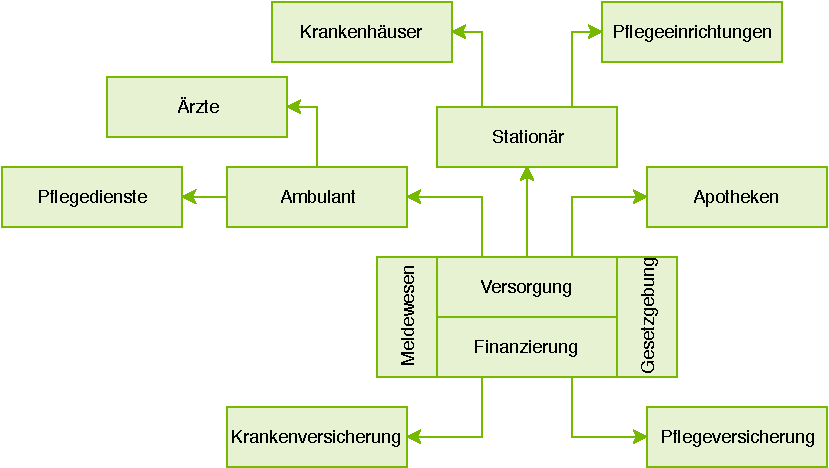
\includegraphics[height=5.5cm]{Bilder/Gesundheitssystem.pdf}
     \caption{Akteure im Gesundheitssystem. Eigene Abbildung in Anlehnung an \cite{SmartHealth}}
   \end{figure}
\end{frame}

\begin{frame}{...und ein kurzer Blick in die Tiefe}
   \begin{figure}[h!]
    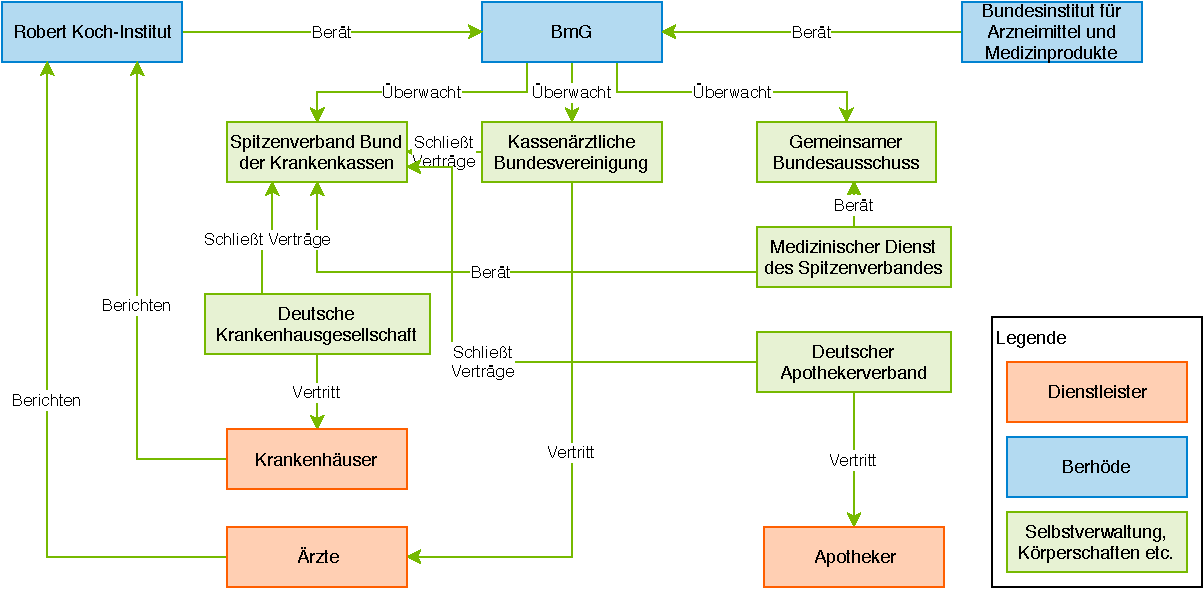
\includegraphics[height=5.5cm, right]{Bilder/GesundheitssystemAkteureBund.pdf}
     \caption{Einige Interaktionen auf Bundesebene. Eigene Abbildung.}
   \end{figure}
\end{frame}

\begin{frame}{Datenaustausch (Beispiel GKV)}
   \note{\begin{itemize}
       \item Richtlinien für den Datenaustausch im Gesundheits- und Sozialwesen, 110 Seiten
       \item Häufig im Einsatz: Mainframe, COBOL
   \end{itemize}}
   \begin{figure}[h!]
    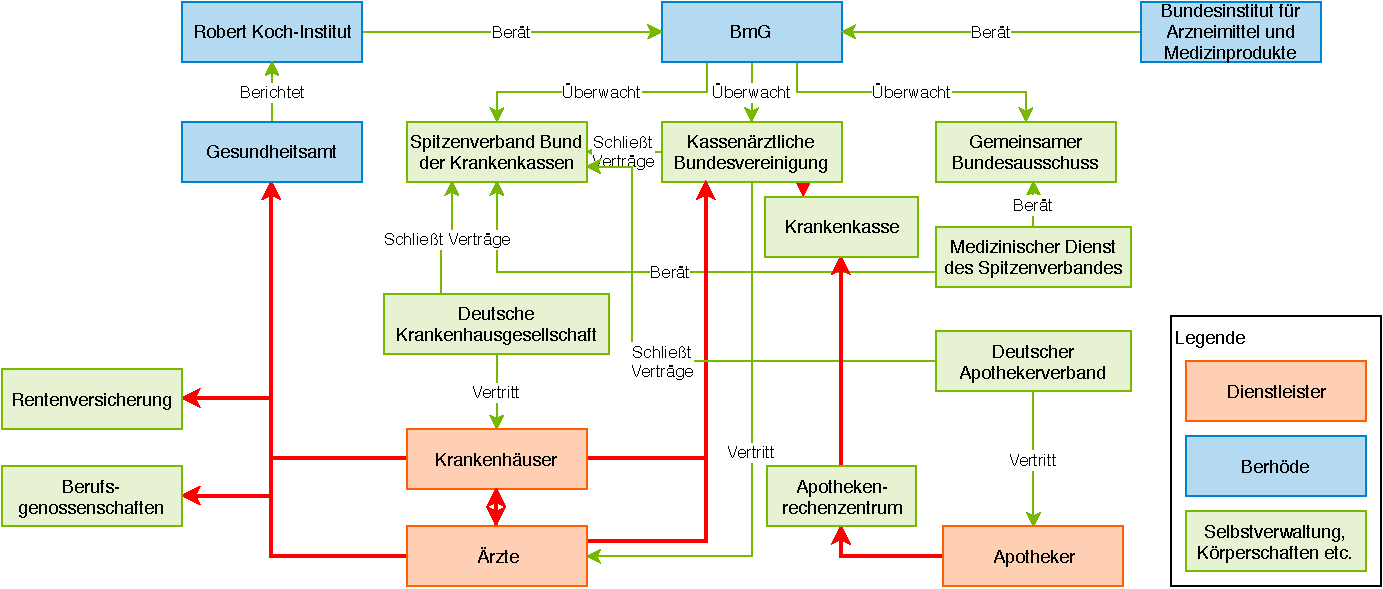
\includegraphics[height=5.5cm, right]{Bilder/DatenfluesseGesundheitssystem.pdf}
     \caption{Beispiele für Austausch personenbezogener Daten im Gesundheitssystem. Eigene Abbildung.}
   \end{figure}
\end{frame}

\begin{frame}{Herausforderungen}
\note{
\begin{itemize}
    \item Steigende Anzahl an Ärzten
    \item Sinkende Zeit pro Patient
    \item Gründe: 
    \begin{itemize}
        \item Demographischer Wandel
        \item Bessere Behandelbarkeit trivialer Erkrankungen führt zu mehr chronischen und komplexen Erkrankungen
        \item<4> Zunehmende Pflegebedürftigkeit
        \item<4> Steigende Dokumentationspflichten
        \item<4> Steigende Komplexität der Diagnose/Behandlung
    \end{itemize}
\end{itemize}}
\begin{minipage}{.4\textwidth}
   \begin{figure}[h!]
    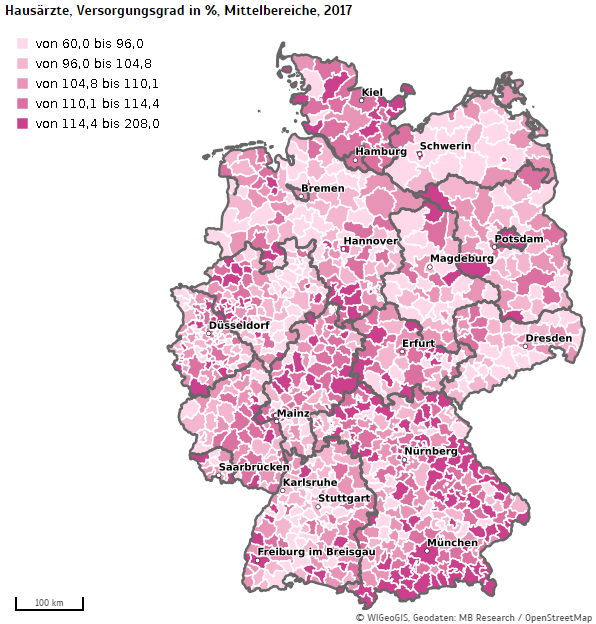
\includegraphics[height=5.5cm, left]{Bilder/HausarztVersorgung.png}
     \caption{Versorgung mit Hausärzten in 2017 \cite{HausarztVersorgung}}
   \end{figure}
   \end{minipage}
  \only<2->{
  \begin{textblock}{10}(6,0.5)
   \begin{figure}[h!]
     \frame{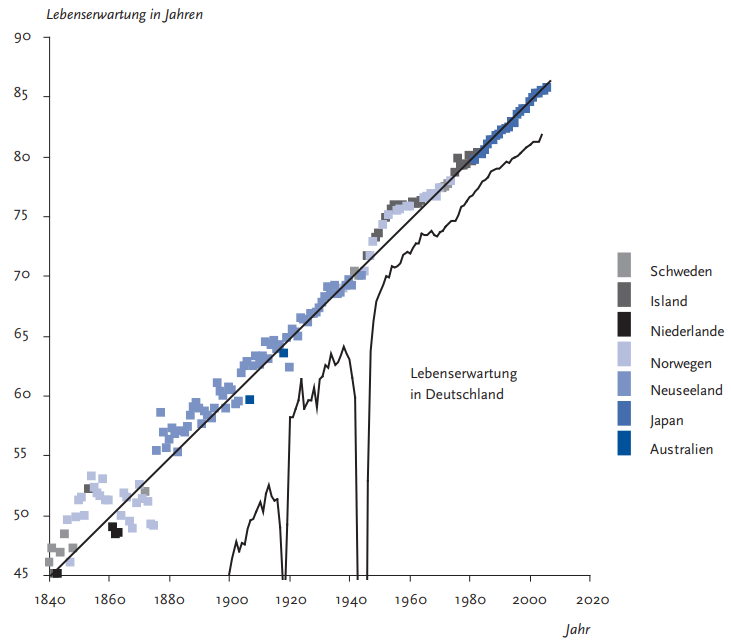
\includegraphics[width=6cm]{Bilder/Rekordlebenserwartungen.PNG}}
     \caption{Anstieg der Rekordlebenserwartung und der Lebenserwartung in Deutschland \cite{GesundheitKrankheitAlter}}
   \end{figure}
  \end{textblock}
  }
  \only<3->{
  \begin{textblock}{10}(6.7,6.7)
   \begin{figure}[h!]
     \frame{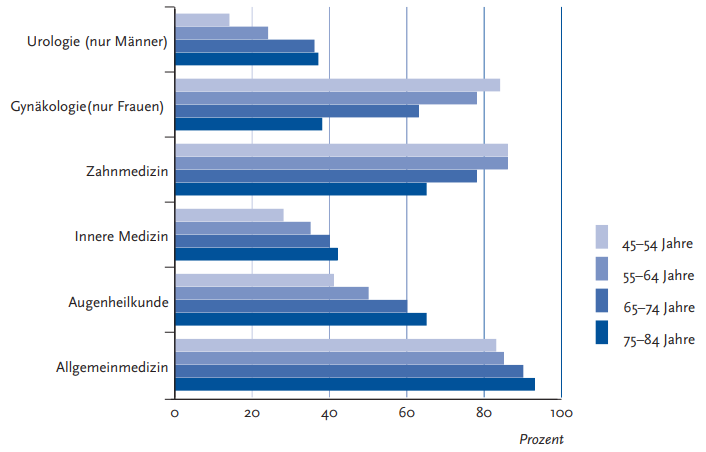
\includegraphics[width=6cm]{Bilder/InanspruchnahmeAerzte.png}}
     \caption{Inanspruchnahme von Ärzten (letzte 12 Monate) nach Alter und Arzt \cite{GesundheitKrankheitAlter}}
   \end{figure}
  \end{textblock}
  }
  \only<4->{
  \begin{textblock}{10}(2.8,3.8)
   \begin{figure}[h!]
     \frame{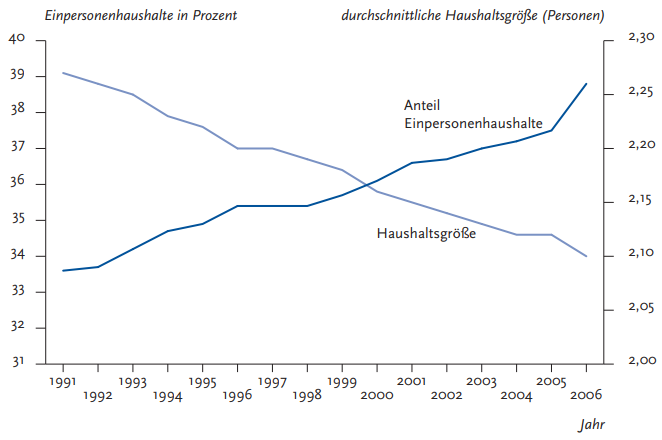
\includegraphics[width=6.5cm]{Bilder/Einpersonenhaushalte.png}}
     \caption{Entwicklung der Haushaltsgröße \cite{GesundheitKrankheitAlter}}
   \end{figure}
  \end{textblock}
 }
\end{frame}

\begin{frame}{Exkurs: Warum Python?}
  \only<2->{Was sind typische Aufgabenbereiche für Bioinformatiker?\vspace{0.3cm}}
  \note<2>{
   Vorsicht:
   \begin{itemize}
       \item Das bezieht sich alles primär auf Bioinformatik
       \item Medizininformatik: 99\% Windows
   \end{itemize}
  }
  \begin{columns}
   \begin{column}{0.5\textwidth}
     \only<3->{\centering \textbf{Softwareentwicklung}}
     \begin{itemize}
       \item<3->Produktzentriert
       \item<3->Performante Implementation eines Algorithmus
       \item<3->Stabilität, Reproduzierbarkeit, gutes User Interface
       \item<4->Primär Java, C++
     \end{itemize}
   \end{column}
   \begin{column}{0.5\textwidth}
     \only<5->{\centering \textbf{Datenauswertung}}
     \begin{itemize}
       \item<5->Projektzentriert
       \item<5->Verwendung existierender Tools
       \item<5->Entwicklung von Pipelines
       \item<5->Implementation kleinerer Algorithmen
       \item<5->Flexibilität, bedarfsgerechte Visualisierung
       \item<6->Primär Python, R
     \end{itemize}
   \end{column}
  \end{columns}
  \note<6>{
   Allgemein: Flexibilität ist wichtig!
   \begin{itemize}
       \item Java super für portable, performante Applikationen, aber mies für Prototyping
       \item Python super für Prototyping, aber schlecht für Stabilität
       \item PHP Totalausfall bei Wartbarkeit+Sicherheit, aber toll für schnelle kleine Webapp
       \item Wünsche JavaScript schnellen und schmerzhaften Tod, setze es trotzdem für interaktive Visualisierungen ein
   \end{itemize}
   Fazit: Keine silver bullet, man muss viele Stärken und Schwächen kennen, und z.T. Programmierkonzepte zwischen Sprachen übertragbar. 
  }
\end{frame}

\begin{frame}{Exkurs: Warum Python (II)?}
  \begin{textblock}{10}(1,2.8)
   \begin{figure}[h!]
     \frame{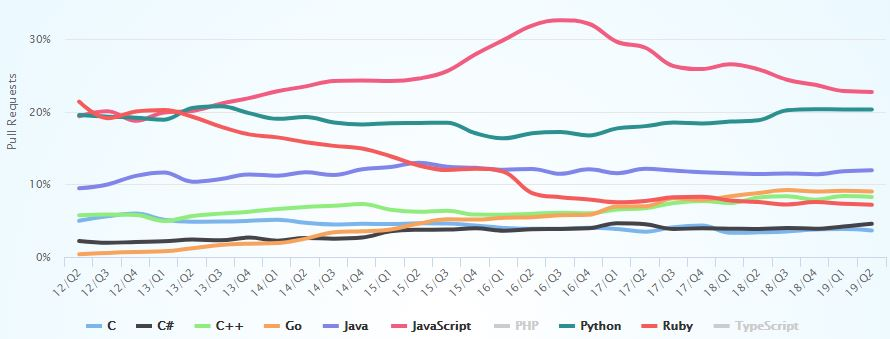
\includegraphics[width=12cm]{Bilder/PythonPulls.jpg}}
     \caption{Pull-requests auf github nach Sprache \cite{PythonPulls}}
   \end{figure}
  \end{textblock}
 \only<2->{
  \begin{textblock}{10}(0.9,3)
   \begin{figure}[h!]
     \frame{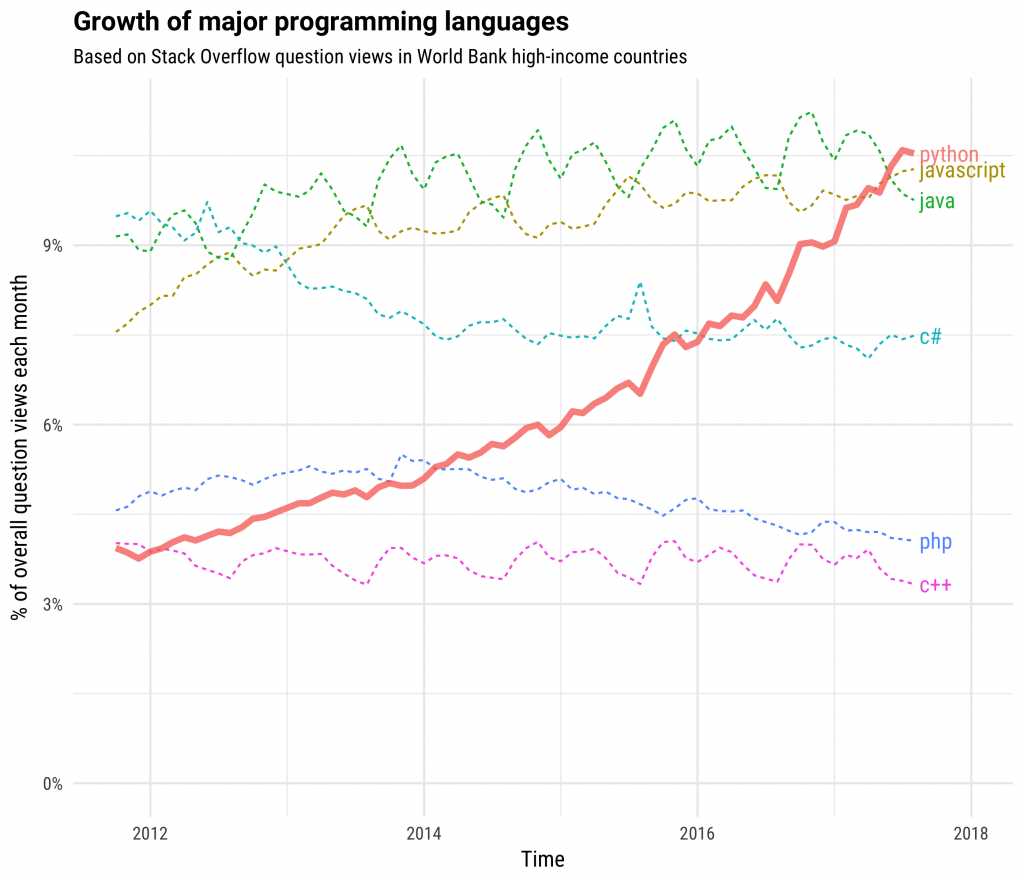
\includegraphics[width=6.5cm]{Bilder/PythonQuestions.png}}
     \caption{Fragen auf StackOverflow nach Sprache \cite{PythonQuestions}}
   \end{figure}
  \end{textblock}
 }
 \only<3->{
  \begin{textblock}{10}(7.1,0.6)
   \begin{figure}[h!]
     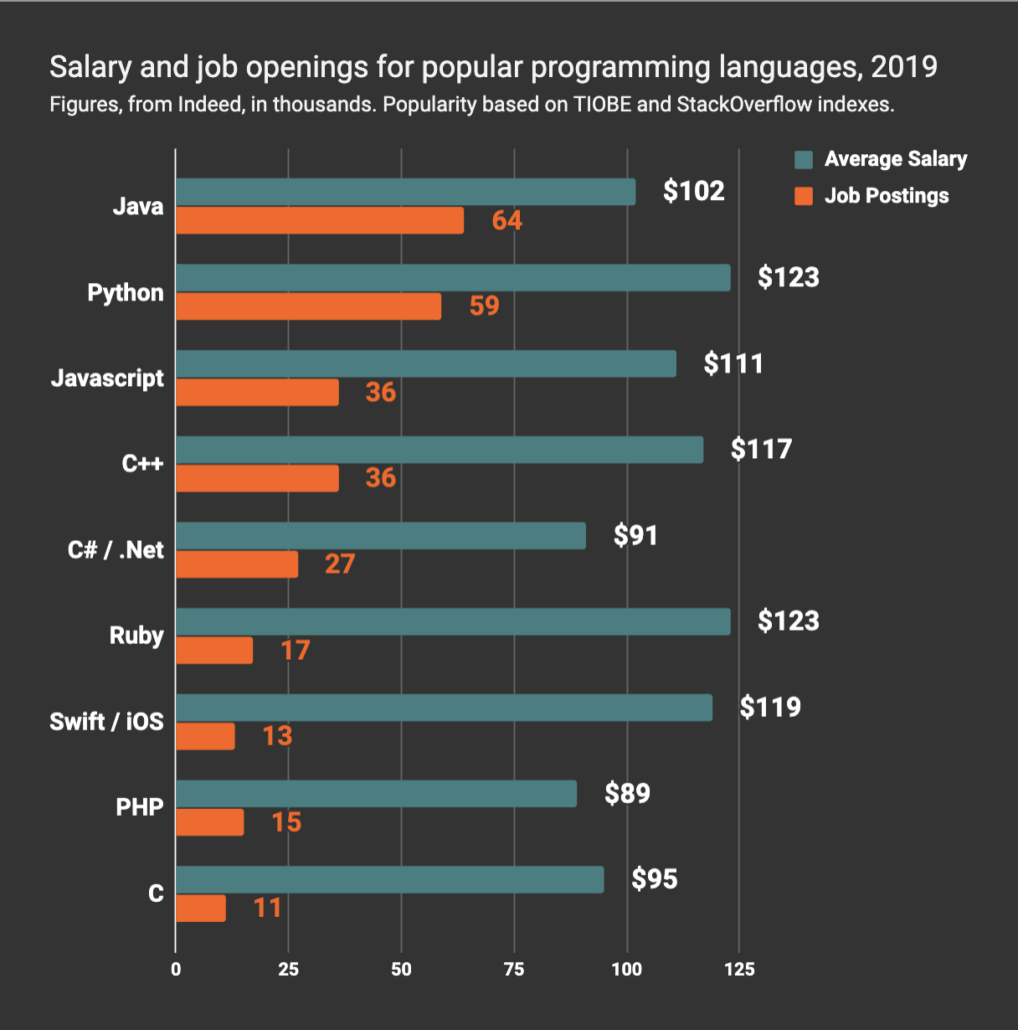
\includegraphics[width=7cm]{Bilder/LanguagesSalary.png}
     \caption{Einkommen und Stellen nach Programmiersprache \cite{LanguagesSalary}}
   \end{figure}
  \end{textblock}
 } 
\end{frame}

\begin{frame}{IT-Unterstützung}
  \note{
  \begin{itemize}
      \item UC: Z.B. Blutdruck, Blutzucker, Sturzsensor, Lokationssensor (Wandern von Alzheimer-Patienten), Schweiß- und Herzfrequenzüberwachung zur Vorhersage epileptischer Anfälle etc.
      \item Benachrichtigung in Stufen, z.B. Angehörige, dann Pflegepersonal
      \item Erinnerung an Medikamente (Problem: Adhärenz!)
      \item Generell: Ortsunabhängige Pflege (zu Hause)
      \item <2-> Automatische Übertragung von Geräten zu zentralen Datenbanken, automatische Vorauswertungen von Bilddaten
      \item<2-> Standardisierung - großes Problem in Medizintechnik
      \item<3-> Abgleich verschriebener Medikamente mit gelber oder roter Liste
      \item<5-> Automatische Benachrichtigung bei Ablauf von Blutkonserven, RFID-Kennzeichnung von OP-Besteck um Desinfektionszyklen einzuhalten etc.
  \end{itemize}}
  \begin{itemize}
      \item Ubquitous Computing: Sensorik und automatische Benachrichtigungen, insbesondere in der Pflege
      \item<2-> Verbesserung der Technikintegration
      \item<3-> Expertensysteme zur Behandlungsunterstützung
      \item<4-> Dokumentationsunterstützung
      \item<5-> Logistik
      \item<6-> Allgemein: Entlastung und Effizienzsteigerung, um bei gleichem Personal mehr Zeit für die Patienten zu haben
  \end{itemize}
\end{frame}

\begin{frame}{Beispiel: Implantateregister}
\note{BfArM: Bundesinstitut für Arzeneimittel und Medizinprodukte}
  \begin{itemize}
      \item Überwachung von Implantaten
      \item Derzeit Vigilanzsystem (Erfassung von Vorfällen), freiwillige wissenschaftliche Register
      \item<2-> Lösung: Verpflichtendes Register zur Qualitätskontrolle und systematischen Auswertungen zur Identifikation niedrigfrequenter Probleme
      \item<3-> Aktueller Stand: Gesetzentwurf vom 3.4.2019
      \item<4-> Komplexe Struktur zur Sicherstellung des Datenschutzes: Vertrauensstelle, Registerstelle, Geschäftsstelle
  \end{itemize}
\end{frame}

\begin{frame}{Datenflüsse im Implantateregister}
   \only<1>{\begin{figure}[h!]
    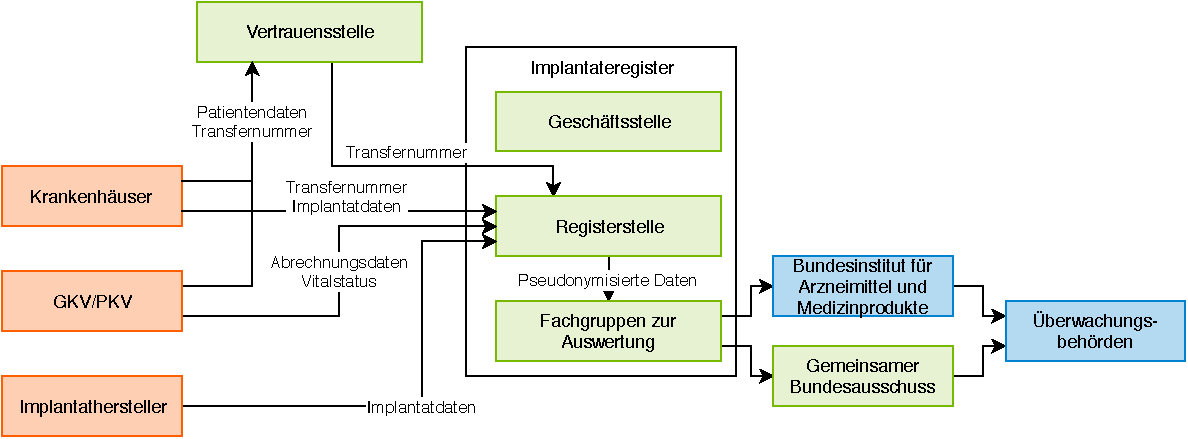
\includegraphics[height=5.5cm, right]{Bilder/Implantateregister.pdf}
     \caption{Dateneinlieferung öim Implantateregister. Eigene Abbildung basierend auf \cite{Implantateregister}}
   \end{figure}
   }
   \only<2>{\begin{figure}[h!]
    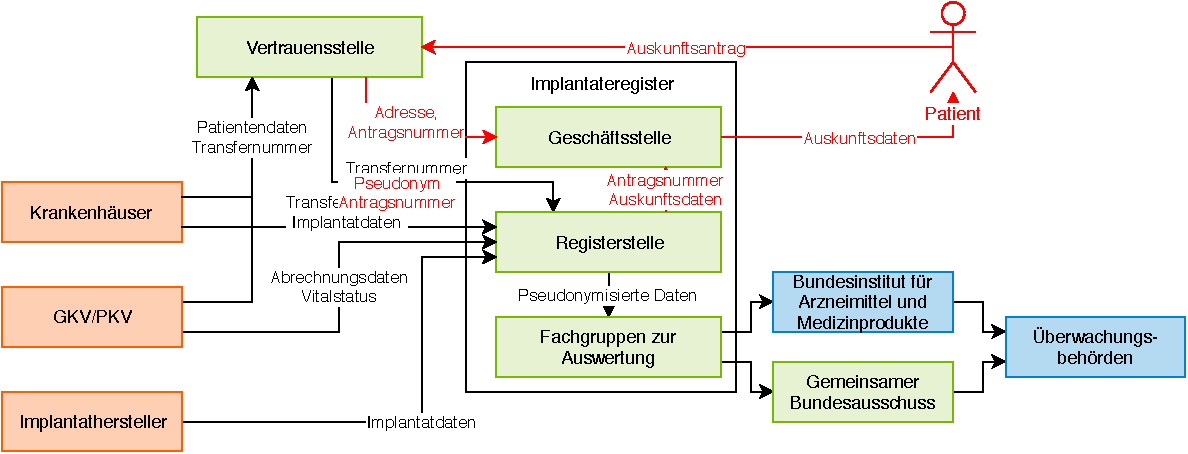
\includegraphics[height=5.5cm, right]{Bilder/ImplantateregisterPatient.pdf}
     \caption{Bearbeitung eines Auskunftsantrags aus dem Implantateregister. Eigene Abbildung basierend auf \cite{Implantateregister}}
   \end{figure}
   }
\end{frame}

\stepcounter{slidesection}
\setbeamertemplate{background}[bgfirst]
\setbeamertemplate{footline}[first]
\subtitle{\theslidesection: Technische Grundlagen}
\titlegraphic{Bilder/logo2.png}
\begin{frame}[noframenumbering]
    \titlepage
    \begin{textblock}{10}(4.75,15)
        \cite{ProgrammingLogo}
    \end{textblock}
\end{frame}
\setbeamertemplate{footline}[presentationbody] 
\setbeamertemplate{background}[bgbody]

\begin{frame}{Sourcecodeverwaltung}
    \note{
        \begin{itemize}
            \item Perforce
            \begin{itemize}
                \item Einsatz in großen Unternehmen (größtes Repo bei Google, 18/20 top-Spieleherstellern, Netflix etc.)
                \item Ändert darunterliegende Technologie nach Bedarf (aktuell git.kompatibel, aber erste Version 10 Jahre vor git)
            \end{itemize}
            \item Subversion: Tracking von Verschieben, Umbenennen etc.
            \item git: Durch Kommerzialisierung von BitKeeper
            \item mercurial: Gleiches Ziel wie git (Linux-Kernel), heutzutagez.B. bei Facebook und Mozilla im Einsatz
            \item Einer der großen heiligen Kriege: git vs. mercurial
            \item Derzeit primär im Einsatz: SVN, Perforce, TFS (zentral), git, mercurial (dezentral)
        \end{itemize}
    }
    \begin{itemize}
        \item Ursprüngliche Herangehensweise: Datei\_final\_final\_realfinal\_12.java...
        \item<2-> 1972: Bell labs, SCCS (source code control system, single user, nur Textdateien)
        \item<3-> 1986: CVS (concurrent version system, zentral, dateibasiert)
        \item<4-> 1995: Helix core (Perforce)
        \item<5-> 2000: SVN (subversion, zentral, verzeichnisbasiert)
        \item<6-> 2004: TFS (team foundation server, Microsoft, zentral/git, verzeichnisbasiert mit bug tracker etc.)
        \item<7-> 2005: git (Linus Torvalds, dezentral, verzeichnisbasiert)
        \item<8-> 2005: mercurial (dezentral, verzeichnisbasiert)
    \end{itemize}
\end{frame}

\begin{frame}{Sourcecodeverwaltung (git)}
    \note{Abgabe von Übungsaufgaben nur als Release-Link in git-Repository}    
    \begin{minipage}{.4\textwidth}
        \begin{figure}[h!]
            \frame{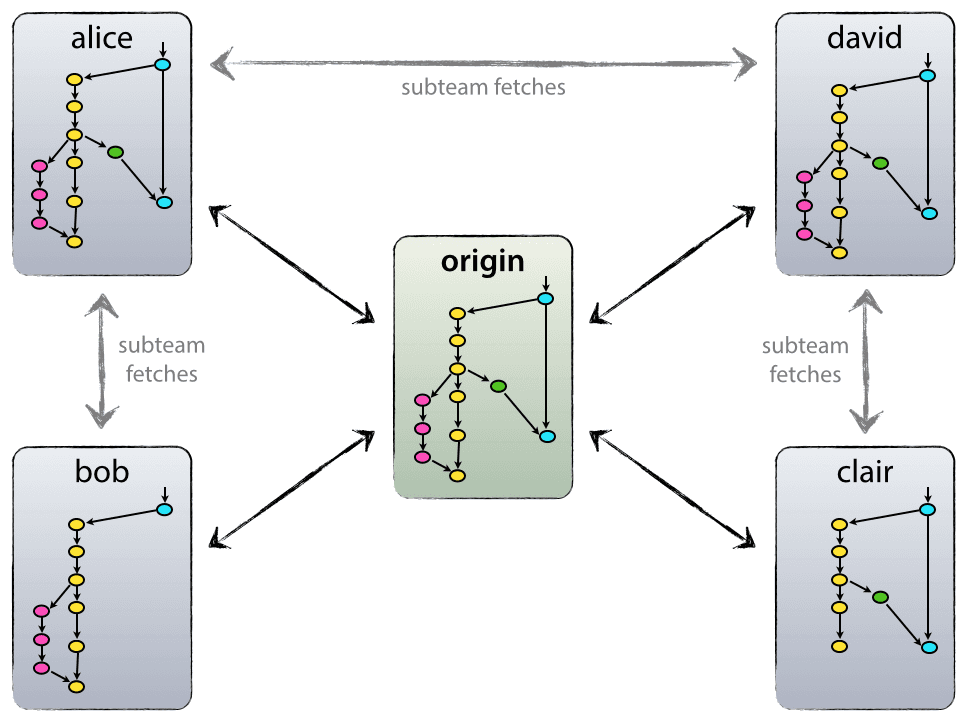
\includegraphics[height=5.5cm]{Bilder/gitbranching2.png}}
            \caption{Teamarbeit mit mehreren remotes \cite{gitbranching}}
        \end{figure}
    \end{minipage}
    \only<2->{
        \begin{textblock}{6}(10,0.2)
            \begin{figure}[h!]
                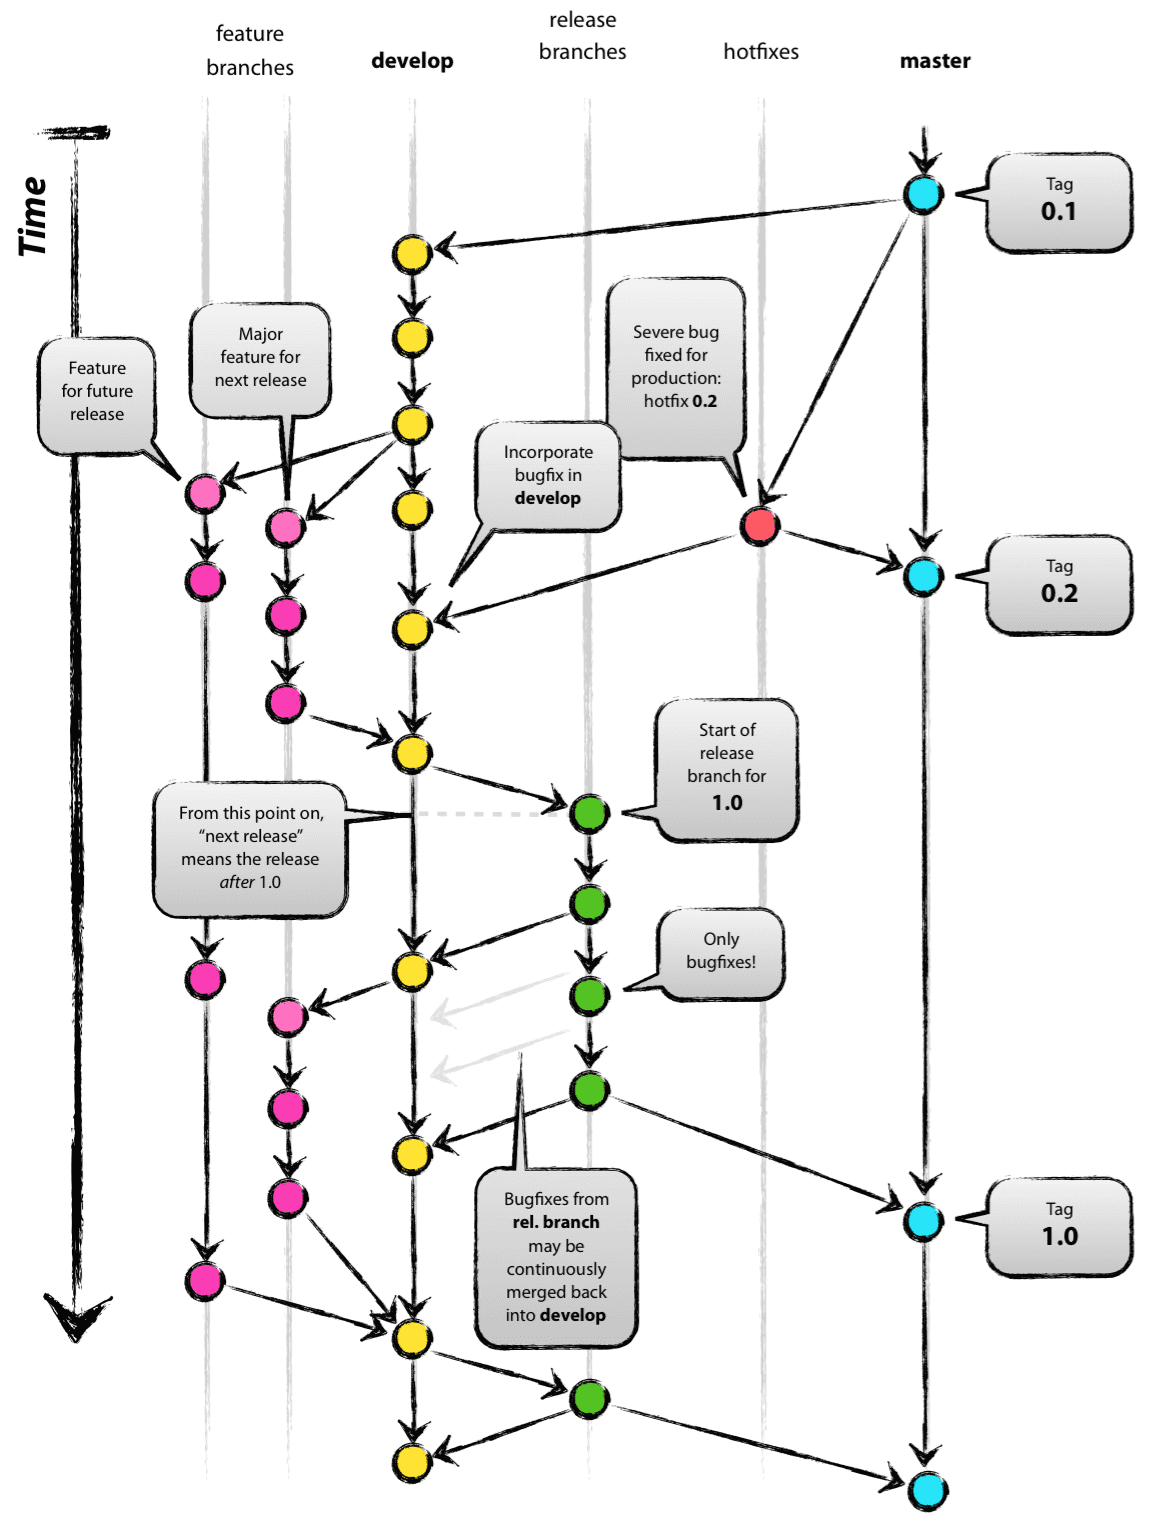
\includegraphics[height=7.3cm, left]{Bilder/gitbranching.png}
                \caption{Komplexe branching-Strategie \cite{gitbranching}}
            \end{figure}
        \end{textblock}
    }
\end{frame}

\begin{frame}{Übung: git}
    \note{
        \begin{itemize}
            \item Gitlab: Open Source (inhouse betreibbar), kostenfreie private Repositories, einfach konfigurierbares CI/CD. Aber grundsätzlich: Geschmackssache.
            \item<3-> Branch-Anpassung
            \item<5-> Abfrage: Ist .git-credentials ein Problem? Hinweisen auf häufige Wiederverwendung von Mail-Passwort-Kombinationen
            \item<7-> \textbf{Diskutieren}: Passwort für key. Ist passwortloser key besser oder schlechter als .git-credentials? Hinweis auf keepass
            \item<8-> \textbf{Diskutieren}: Ist git push --force nach reset auf gepushten commit  eine gute Idee?
        \end{itemize}
    }
    \begin{itemize}
        \item Erstellung eines gitlab-Accounts
        \item<2-> Neues Projekt erstellen, README anpassen (online)
        \item<3-> clone, README anpassen, commit
        \item<4-> push... Aber wo geht es hin? git remote! Und was geht da hin? git branch
        \item<5-> Credentials merken...
        \item<6-> ...und gleich wieder löschen! 
        \item<7-> Alternative: \href{https://docs.gitlab.com/ee/ssh/}{SSH-Key}. Dafür: clone über SSH (oder remote anpassen?)
        \item<8-> Fehler rückgängig machen: git reset (vor und nach push)
    \end{itemize}
\end{frame}


\begin{frame}[fragile]{\only<1-4,6->{Python}}
    \note{
        \begin{itemize}
            \item Unterschiede compiliert and linked, interpretiert (bytecode), JIT
            \item Source code $\rightarrow$ Object code $\rightarrow$ Executable
        \end{itemize}
    }
    \begin{itemize}
        \item Interpretierte Sprache
        \item<4-> Multi-paradigm: Objektorientiert, mit funktionalen Elementen
        \item<4-> Typisierung: Dynamisch, stark (dynamically, strongly typed)
        \item<6-> Automatisches Speichermanagement
        \item<7-> Designziel: Einfach zu lesen und zu schreiben, prägnant (wenig boilerplate code)
        \item<7-> Einrückung statt Klammern
    \end{itemize}
    \only<2>{
        \begin{textblock}{10}(3,0.2)
            \begin{figure}[h!]
                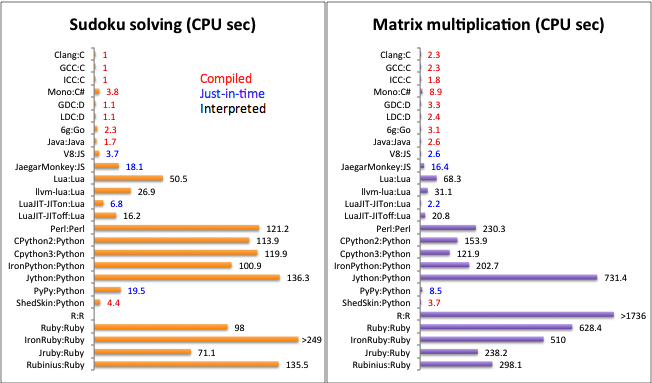
\includegraphics[height=7.3cm, left]{Bilder/langperformance.png}
                \caption{Beispielhafter Performance-Vergleich zwischen Sprachen \cite{langperformance}}
            \end{figure}
        \end{textblock}
    }
    \only<3> {
        \begin{textblock}{10}(2,4)
            \begin{figure}
                \lstinputlisting[frame=single, language=Python, backgroundcolor = \color{white}]{Uebungen/hello.py}
                \caption{Beispiel für Laufzeitfehler}
            \end{figure}
        \end{textblock}    
    }
    \only<5> {
        \begin{figure}
            \begin{textblock}{14}(1,0.5)
                \lstinputlisting[frame=single, language=Python, backgroundcolor = \color{white}]{Uebungen/types.py}
            \end{textblock}    
            \begin{textblock}{14}(1,5.5)
                \lstinputlisting[frame=single, language=Java, backgroundcolor = \color{white}]{Uebungen/types.java}
                \caption{Java und Python: Schwache und starke Typisierung}
            \end{textblock}    
        \end{figure}
    }
\end{frame}

\begin{frame}{Python: Einführende Übungen}
    \begin{itemize}
        \item Übungs-repository auf github: \href{https://github.com/dabrowskiw/UE-EinfuehrungGesundheitsinformatik}UE-EinfuehrungGesundheitsinformatik von dabrowskiw
        \item Erster Schritt: Fork in eigenes Gitlab-Repo
    \end{itemize}
\end{frame}


\begin{frame}[allowframebreaks]{Bildquellen}
\printbibliography
\end{frame}

\begin{frame}{Lizenz}
    \begin{center}
        
\includegraphics{Bilder/by.png}\\
        Alle Inhalte außer dem HTW-Logo, für die keine Quelle angegeben ist, sind eigenes Material und unter CC-BY 4.0\\
        \url{https://creativecommons.org/licenses/by/4.0/}\\
        lizenziert.\\\vspace{0.5cm}
        Sämtliche Nutzungs- und Verwertungsrechte für das Logo der HTW Berlin in allen hier verwendeten Formen liegen ausschließlich bei der HTW Berlin:\\
        \url{https://corporatedesign.htw-berlin.de/logos/logo-htw-berlin/}
    \end{center}
\end{frame}

\end{document}
